\section{Feedback Configurations} \label{sec:feed}

The fundamental interest of this project was to develop two novel, intuitive and useful feedback schemes to convey proprioceptive information through electrotactile stimulation and evaluate which one would aid control the most. This was to be implemented in a two DoF virtual prosthesis using wrist rotation and hand aperture as motions, where five levels of sensory feedback would be provided for each DoF to communicate prosthetic position states. 

The center electrode pads were placed most central on the dorsal side of arm. See illustration in \figref{fig:meth:elec_place}. The electrode array was fixated on the non-dominant arm such that there was a maximum gap of three cm between the outer electrode pads volarly. It was chosen to place the electrode array on the non-dominant arm since the electrode pads used did not prohibit current leakage. Thus, placing the electrode on the same arm as the MYB could have resulted in interference, which might corrupt recorded EMG data and impair the control system. Providing feedback to non-dominant arm has, however, proven usable for providing meaningful artificial proprioceptive feedback \cite{Pistohl2015}.  

\begin{figure}[H]                 
	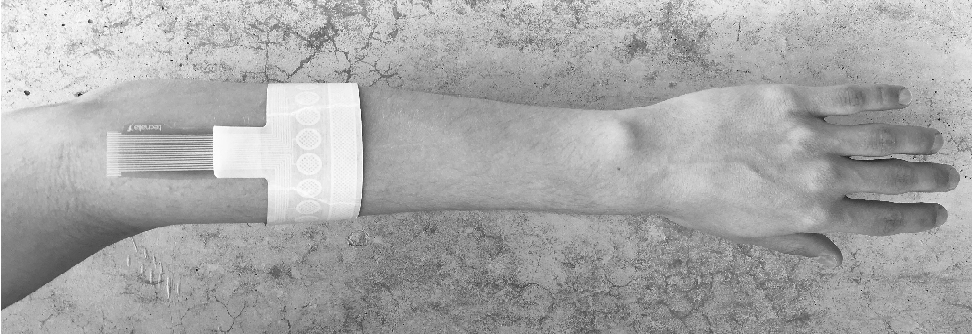
\includegraphics[width=0.85\textwidth]{figures/elec_place}  
	\caption{Illustration of the placement of the electrode array. There was a maximum gap of three cm between the outer electrode pads volarly.}
	\label{fig:meth:elec_place} 
\end{figure} 
The following sections will present the two developed spatial and amplitude feedback schemes. 

\subsection{Spatial Configuration}

The spatial feedback scheme was created with the interest of achieving an intuitive way to convey the feedback by focusing stimulation to localized regions on the skin. An illustration of the spatial feedback scheme can be seen in \figref{fig:spatial}. The idea behind this configuration was to communicate wrist rotation movements by rotating the activated electrode pads and to convey the hand aperture by narrowing distance between active pads. 

To achieve this, the electrode pads were broken into two groups: one upper and one lower. The upper eight pads (5-12) were used to convey information of the rotational DoF using four pads for either side.  The four pads were divided into pairs of two, where the first from the center in e.g. pronation would be activated when the cursor entered the first level position state. Likewise, the second level pair would be activated when the cursor entered the second level. Hence, during a transition from neutral to level one and level one to level two, the subject should feel the stimulation moving either laterally or medially depending on the position state. For subjects with the electrode array fitted on the left arm, this meant that when the virtual prosthesis was in a supinated state the stimulation should be felt in the dorsal medial region of the arm, while when the virtual prosthesis was in a pronated state stimulation should be felt in the dorsal lateral region of the arm.   

The lower eight pads (1-4 and 13-16) were used to convey information about the hand aperture. The pads were paired in an opposite manner for each of the four levels respectively: 4 and 13; 3 and 14; 2 and 15; 1 and 16. As the state would change to one hand aperture state out of four possible, a certain pad pair would activate. Transitioning from neutral to fully closed, the subject should sense the stimulation converging on the volar side of the arm. The virtual prosthesis was able to be in states, which was a combination of the two DoF's. In these cases the feedback would be a combination of any upper and lower pair, resulting in the activation of four pads simultaneously. %In the spatial feedback scheme, it was chosen to use the second amplitude level determined to enhance the subject's perception of the stimuli. (Move to determination of sensory thresholds. The same information in the amplitude scheme should be moved to that section too.)

\begin{figure}[H]                 
	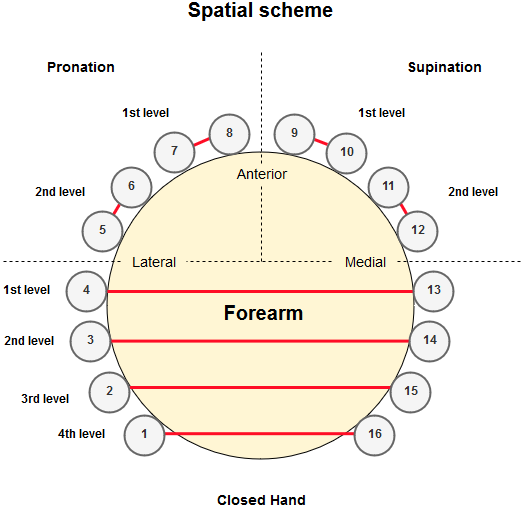
\includegraphics[width=0.55\textwidth]{figures/El_array_spatial}  
	\caption{Transverse view of the developed spatial scheme, which was based on different pads being activated depending on the level of the position state. The level assigned to the various electrode pairs corresponded to levels of position states in \figref{fig:meth:gridmap}. The highest number of possibly activated pads was four at a time. For subjects with the electrode array fitted on the right arm the rotational states were reversed.}
	\label{fig:spatial} 
\end{figure}


\subsection{Amplitude Configuration}

In this scheme, attention to the recognition of stimulation localization should be less. Instead, the subject would have to discriminate between the intensity of stimulation in the regions which were active. 

Compared to the spatial configuration where the feedback was given through dynamically changing the pads activated, the amplitude configuration instead conveyed feedback in three greater regions and solely modulated the amplitude of the stimulation. The upper eight pads were again used for the rotational DoF, illustrated in \figref{fig:amplitude}. Pads 5-8 were activated with different amplitude levels at pronated states 1 and 2, respectively. The same was applicable for supinated states using pads 9-12. 

For conveying information about hand aperture, pads 1,2,15 and 16 were used. When in a combined DoF position state, eight pads would be active in amplitude levels relative to the level of the state. It was chosen to use groups of four electrode pads to exploit the largest number of pads in the electrode array, while still maintaining a symmetric distribution of possible active pads.

\begin{figure}[H]                 
	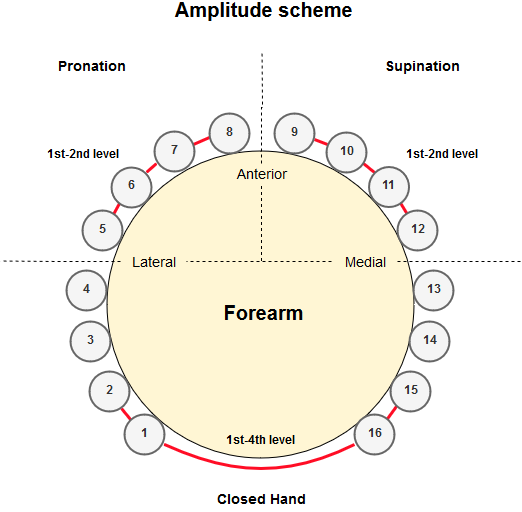
\includegraphics[width=0.55\textwidth]{figures/El_array_amplitude}  
	\caption{Transverse view of the developed amplitude scheme. Here, the amplitude of the active pads would increase with the increase of the position state; the higher the level the higher the current amplitude of the given pads. The level of amplitude strength assigned to the various pads corresponded to levels of position state in \figref{fig:meth:gridmap}. The highest number of possibly activated pads was eight at a time.  For subjects with the electrode array fitted on the right arm the rotational states were reversed.}
	\label{fig:amplitude} 
\end{figure}






